\documentclass[a4paper,12pt]{article} % добавить leqno в [] для нумерации слева
\usepackage[a4paper,top=1.3cm,bottom=2cm,left=1.5cm,right=1.5cm,marginparwidth=0.75cm]{geometry}
%%% Работа с русским языком
\usepackage{cmap}					% поиск в PDF
\usepackage{mathtext} 				% русские буквы в фомулах
\usepackage[T2A]{fontenc}			% кодировка
\usepackage[utf8]{inputenc}			% кодировка исходного текста
\usepackage[english,russian]{babel}	% локализация и переносы

\usepackage{graphicx}

\usepackage{wrapfig}
\usepackage{tabularx}

\usepackage{hyperref}
\usepackage[rgb]{xcolor}
\hypersetup{
colorlinks=true,urlcolor=blue
}
\usepackage{multirow}
\usepackage{hhline}


%%% Дополнительная работа с математикой
\usepackage{amsmath,amsfonts,amssymb,amsthm,mathtools} % AMS
\usepackage{icomma} % "Умная" запятая: $0,2$ --- число, $0, 2$ --- перечисление

%% Номера формул
\mathtoolsset{showonlyrefs=true} % Показывать номера только у тех формул, на которые есть \eqref{} в тексте.

%% Шрифты
\usepackage{euscript}	 % Шрифт Евклид
\usepackage{mathrsfs} % Красивый матшрифт

%% Свои команды
\DeclareMathOperator{\sgn}{\mathop{sgn}}

%% Перенос знаков в формулах (по Львовскому)
\newcommand*{\hm}[1]{#1\nobreak\discretionary{}
{\hbox{$\mathsurround=0pt #1$}}{}}

\begin{document}

\newenvironment{lines}[1][\textwidth] % по умолчанию линейки на всю ширину текста
{
\newcolumntype{E}{>{}p{#1}<{\hrulefill}} % в конце нашего столбца будет приписываться \hrulefill
\begin{flushright} % автоматически вставим flushright
\begin{tabular}[h]{E} % и tabular нужного формата
}
{\end{tabular}\end{flushright}
}
	
	\begin{titlepage}
	\begin{center}
		{\large МОСКОВСКИЙ ФИЗИКО-ТЕХНИЧЕСКИЙ ИНСТИТУТ (НАЦИОНАЛЬНЫЙ ИССЛЕДОВАТЕЛЬСКИЙ УНИВЕРСИТЕТ)}
	\end{center}
	\begin{center}
		{\large Физтех-школа электроники, фотоники и молекулярной физики}
	\end{center}
	
	
	\vspace{4.5cm}
	{\huge
		\begin{center}
			Фотоэлектрический способ преобразования энергии солнечного
излучения
		\end{center}
	}
	\vspace{2cm}
	\begin{flushright}
		{\LARGE Салтыкова Дарья \\
			\vspace{0.5cm}
			Б04-104}
	\end{flushright}
	
	\vspace{0.5cm}
	
	\begin{lines}[.5
	\textwidth]
  
\end{lines}
	\vspace{8cm}
	\begin{center}
		Долгопрудный 2024
	\end{center}
\end{titlepage}

\section{Цель работы} 
1.	Исследование темновой и световой вольтамперных характеристик фотоэлемента.
2.	Изучение влияния мощности падающего излучения на характеристики образца с помощью фильтров


\section{Теоретические сведения}
Прямое преобразование лучистой энергии Солнца в электрическую осуществляется с помощью фотоэффекта на потенциальном барьере или так называемого вентильного фотоэффекта, суть которого — возникновение фото-ЭДС при освещении контактов металл-полупроводник и p-n переходов. Однако, вследствие сложной микроструктуры контактов полупроводника с металлом, мы ограничимся в дальнейшем наиболее ясным случаем p-n переходов.

\begin{figure}[h!]
    \centering
    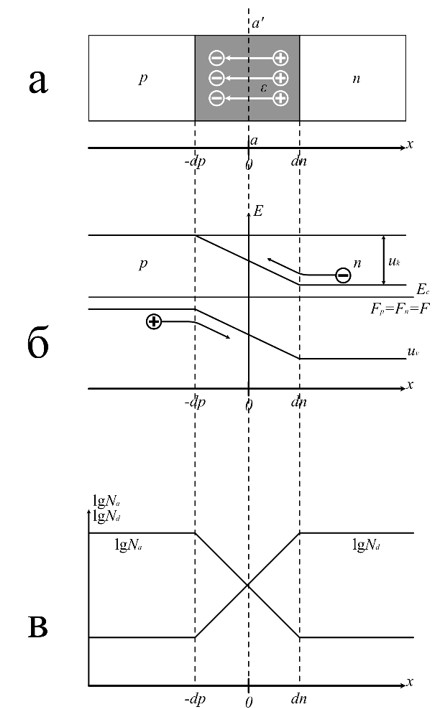
\includegraphics[scale=0.5]{1.1.jpg}
    \caption{Схема p-n перехода}
\end{figure}

Рассмотрим более подробно, что представляет собой p-n переход. Пусть два полупроводника, один из которых имеет проводимость p-типа, а другой n-типа приводятся в хороший контакт по плоскости $aa'$, как показано на изображении а (Рисунок 1). Тогда под действием градиента концентрации дырки из приконтактного слоя p-области будут диффундировать в n-область, а электроны из приконтактного слоя n-области — в p-область. В результате такой диффузии в приконтактном слое p-области создается отрицательный объёмный заряд нескомпенсированных ионов акцепторной примеси, а в приконтактном слое n-области — положительный объёмный заряд нескомпенсированных ионов донорной примеси. 

Порожденное объёмными зарядами электрическое поле (направление которого показано на изображении а (Рисунок 1)), будет препятствовать дальнейшей диффузии основных носителей зарядов (основными называются носители, знак которых соответствует типу проводимости полупроводника). При этом напряжённость электрического поля $\vec{\varepsilon}$ и толщины слоёв объёмных зарядов в $n$ и $p$-областях будут возрастать до тех пор, пока не достигнут своих равновесных значений $\vec{\varepsilon_0}$, $d_p$ и $d_n$, при которых диффузионные потоки основных носителей зарядов полностью скомпенсированы дрейфовыми потоками, вызванными электрическим полем объёмных зарядов. 

Переходная область толщины $d = d_p + d_n$, объединённая свободными носителями зарядов, и в которой локализовано электрическое поле с напряжённостью $\vec{\varepsilon_0}$, получила название электронно-дырочного или $p$-$n$-перехода. Толщина $p$-$n$-перехода $d$ для различных полупроводниковых систем может изменяться от единицы до сотых долей микрометров, а величина $\vec{\varepsilon_0}$ достигать значений $\sim 10^7 \, \text{В}\cdot\text{см}^{-1}$.

Состояние $p$-$n$-перехода в термодинамическом равновесии легко понять, обращаясь к его энергетической диаграмме, приведённой на схеме б (Рисунок 1). Здесь $E_c$ — дно зоны проводимости, $E_v$ — потолок валентной зоны, $F$ — уровень Ферми. В самом деле, электроны из $n$-области не могут проникнуть в $p$-область, так как для этого им необходимо преодолеть потенциальный барьер, высота $u_k$ которого равна контактной разности потенциалов, а энергия электронов меньше высоты этого барьера. По аналогичной причине дырки из $p$-области не могут попасть в $n$-область.

На практике $p$-$n$-переходы реализуются не механическим соединением двух полупроводников, а внутри единого кристалла, в котором создают подходящее распределение донорной $N_d$ и акцепторной $N_a$ примесей, как показано на схеме в (Рисунок 1).



\section{Схема установки}

\begin{figure}[h!]
    \centering
    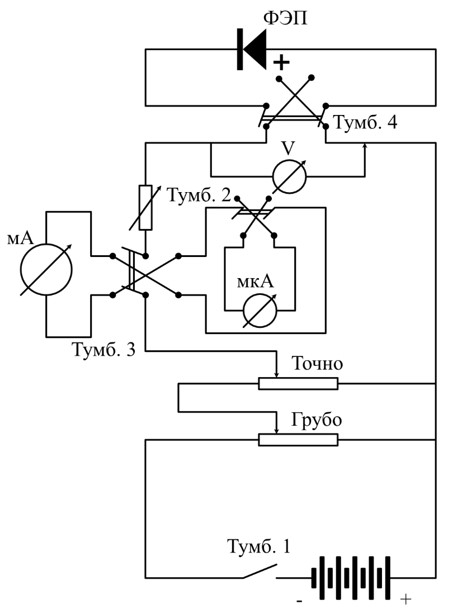
\includegraphics[scale=0.5]{1.jpg}
    \caption{Экспериментальное установка}
\end{figure}

Вольтамперная характеристики фотопреобразователя могут быть измерены с помощью схемы, представленной на схеме (Рисунок 2). Когда преобразователь работает как генератор электроэнергии, то в качестве источника излучения используется лампа марки 3H7 или 3Н8 с встроенным зеркальным отражателем и мощностью 500 Вт. Спектр ее излучения с помощью водяного фильтра приближен к спектру солнечного излучения и к спектральной чувствительности кремниевого преобразователя.

\section{Ход работы}
\subsection{Первая установка}

Построим график прямой ветви теневой вольт-амперной характеристики.

\begin{figure}[h!]
    \centering
    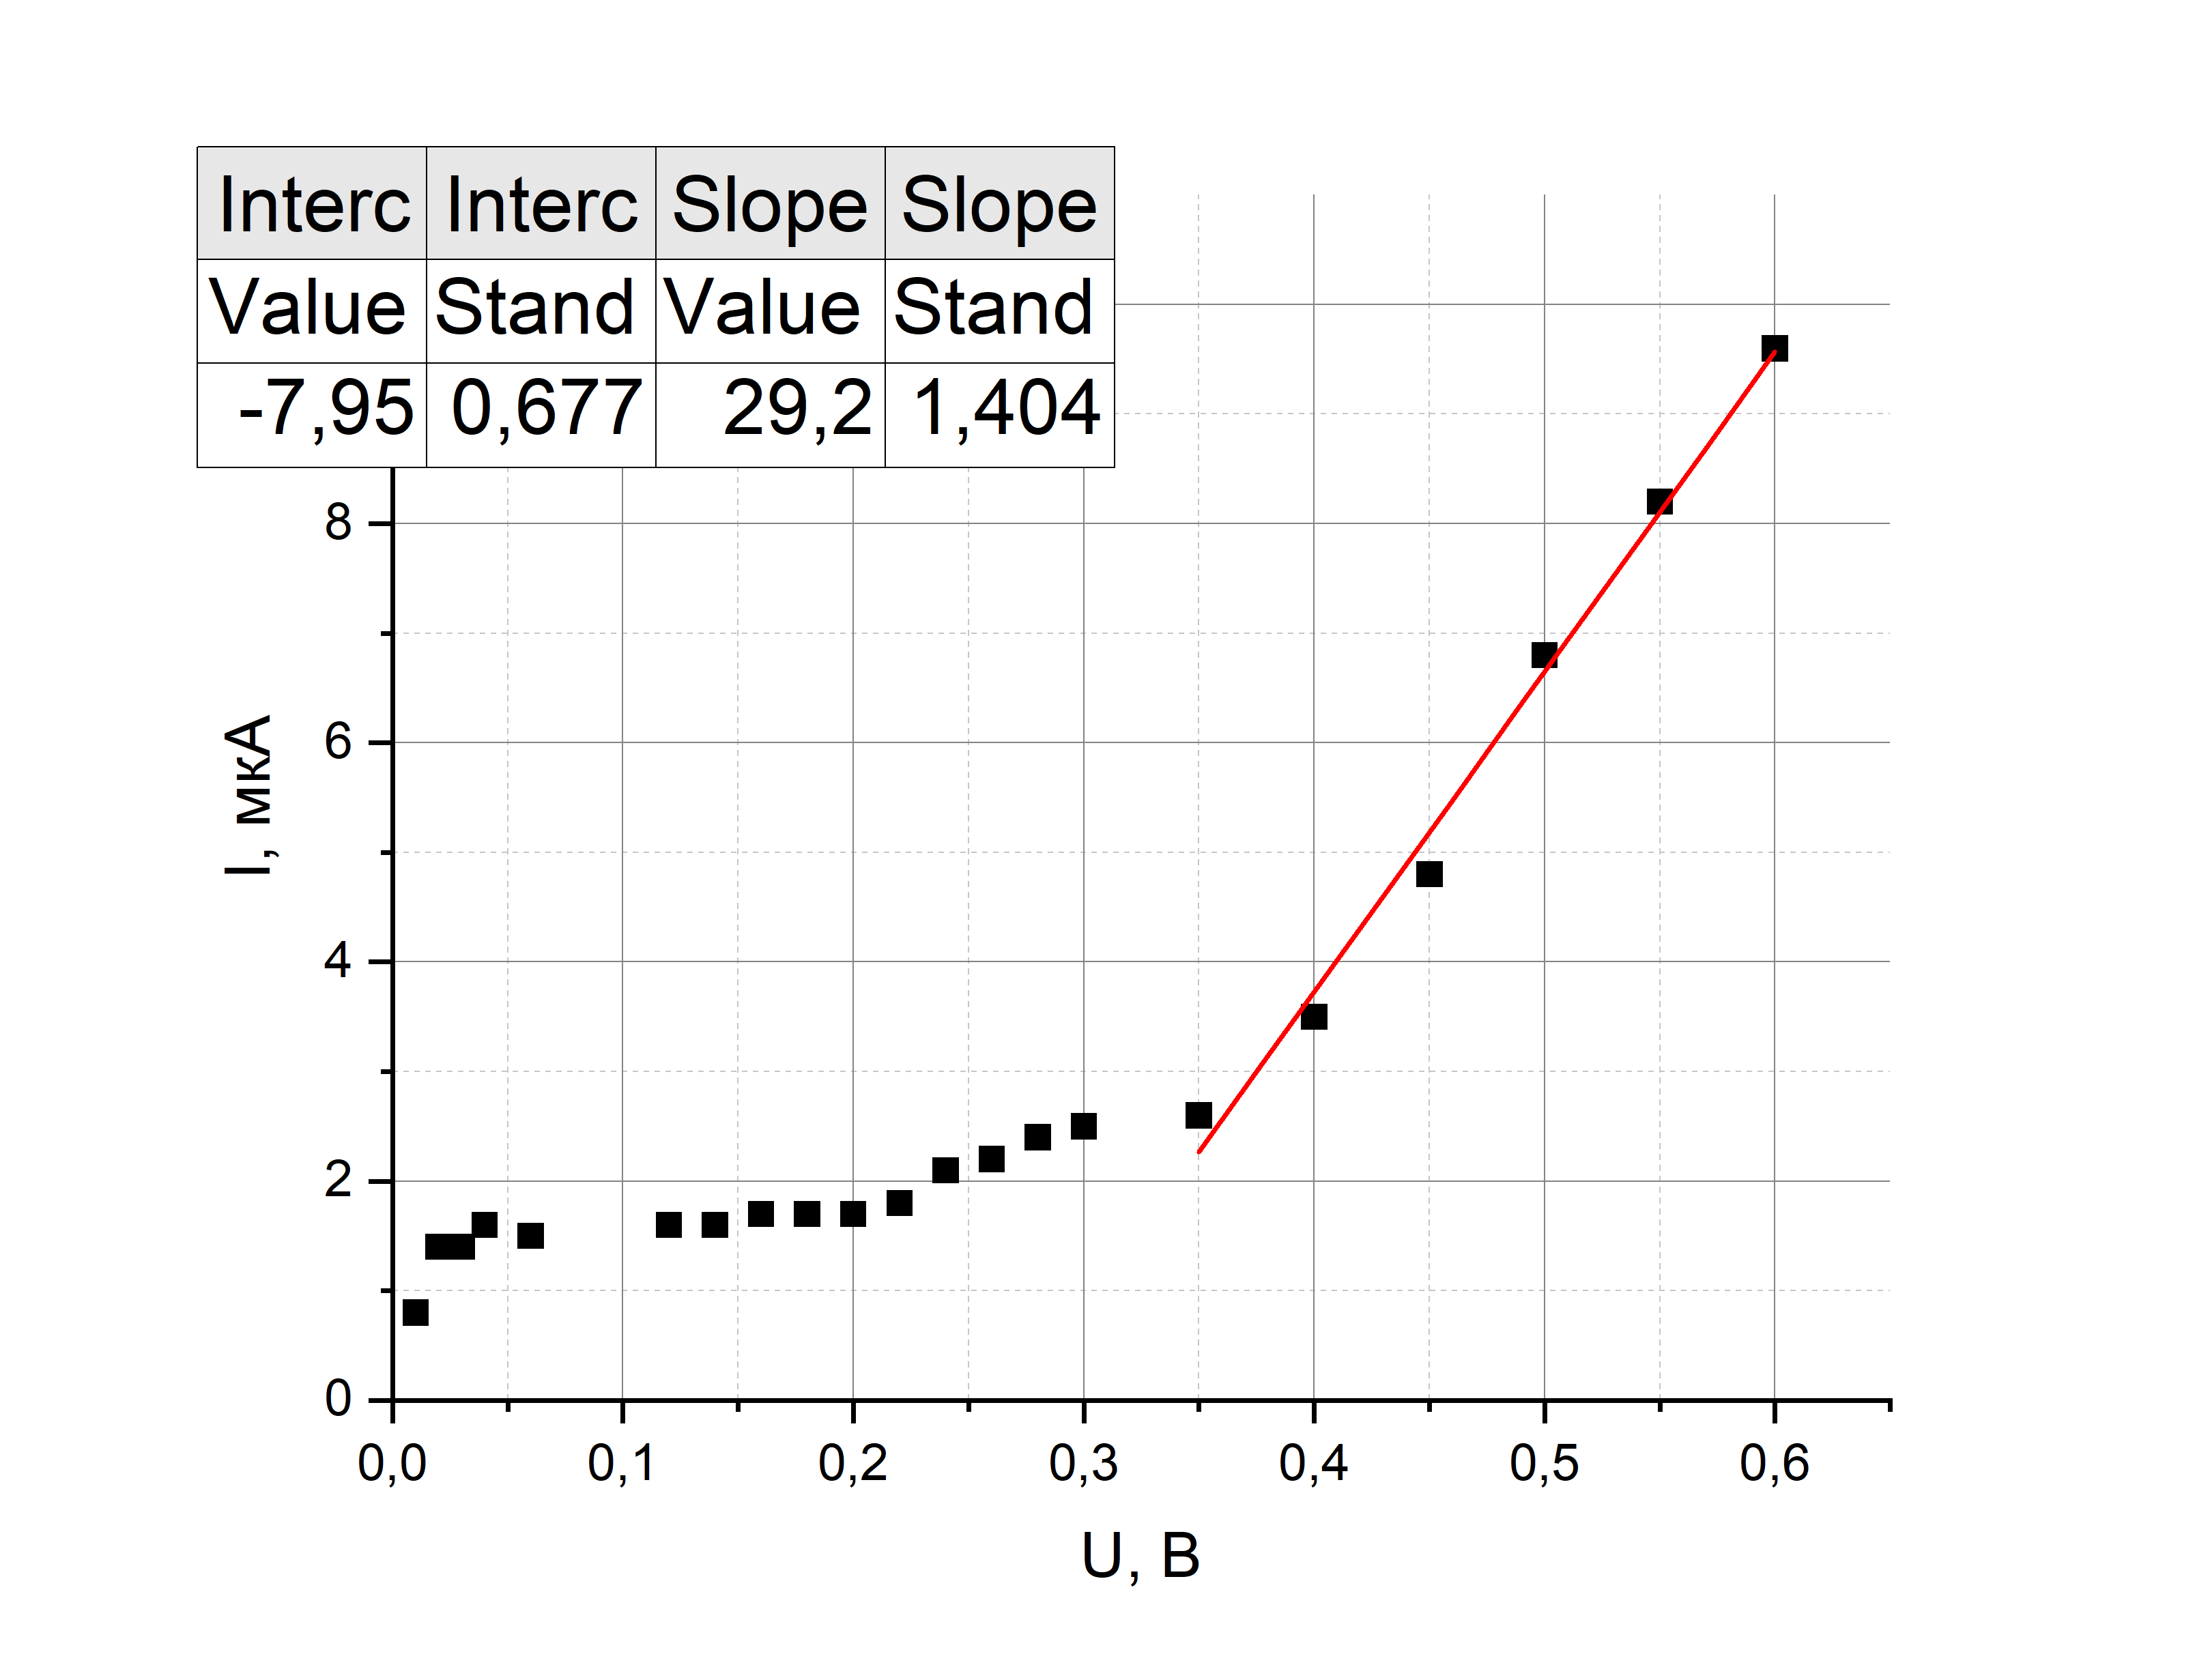
\includegraphics[scale=0.5]{прямая темновая.png}
    \caption{Прямая темновая характеристика фотоэлемента}
\end{figure}


Определим по нему прямое сопротивление элемента:

\[
R_{\text{пр}} = \frac{dU_{\text{пр}}}{dI_{\text{пр}}} = \frac{1}{a} \approx 34 \pm 2 \, \Omega
\]

Построим зависимость $ln(I)=f(U)$.

\begin{figure}[h!]
    \centering
    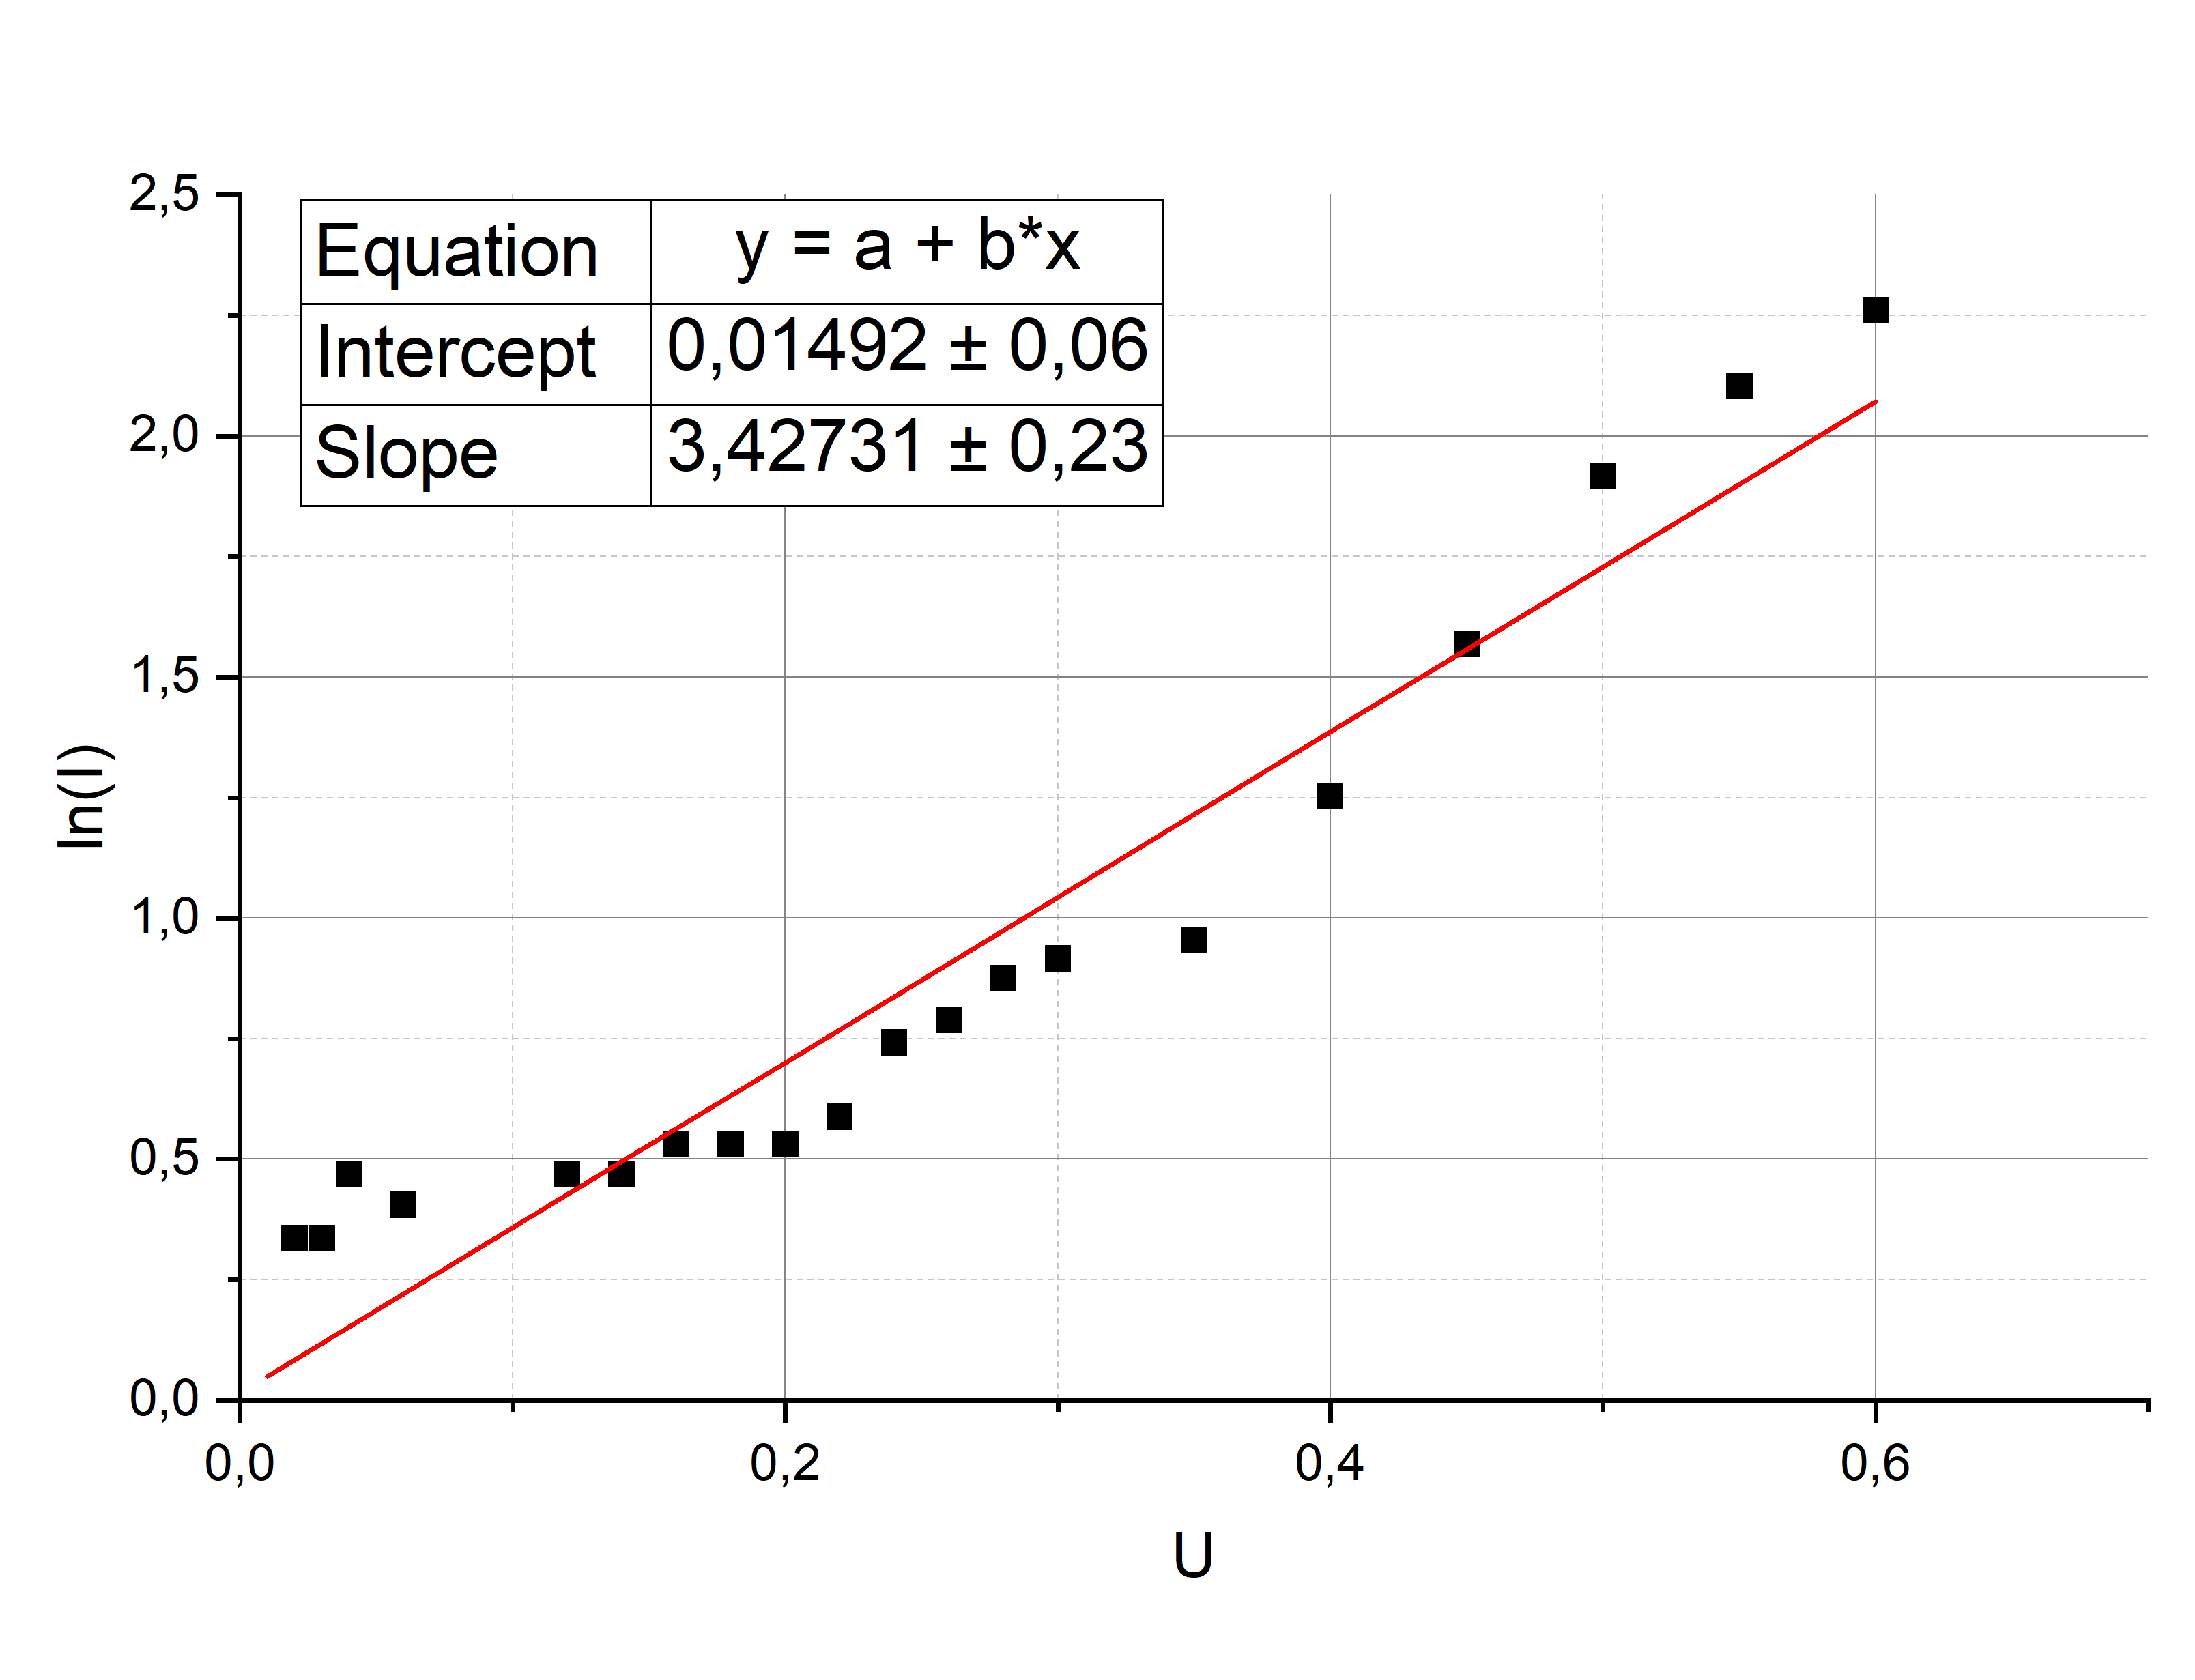
\includegraphics[scale=0.5]{пр темн лог.png}
    \caption{Логарифм прямой темновой характеристики фотоэлемента}
\end{figure}

Определим параметры $A$ и $I_s$:

\[
A = \frac{1}{0.025a} = 11.7 \pm 0.6 \, \frac{1}{\mu A} \quad (2)
\]
\[
I_s = e^b = 1 \pm 0.1 \, \mu A
\]

\subsection{Вторая установка}

Для другого фотоэлемента построим световые характеристики без фильтра и с красным фильтром.

\subsubsection{Световая характеристика без фильтра}

\begin{figure}[h!]
    \centering
    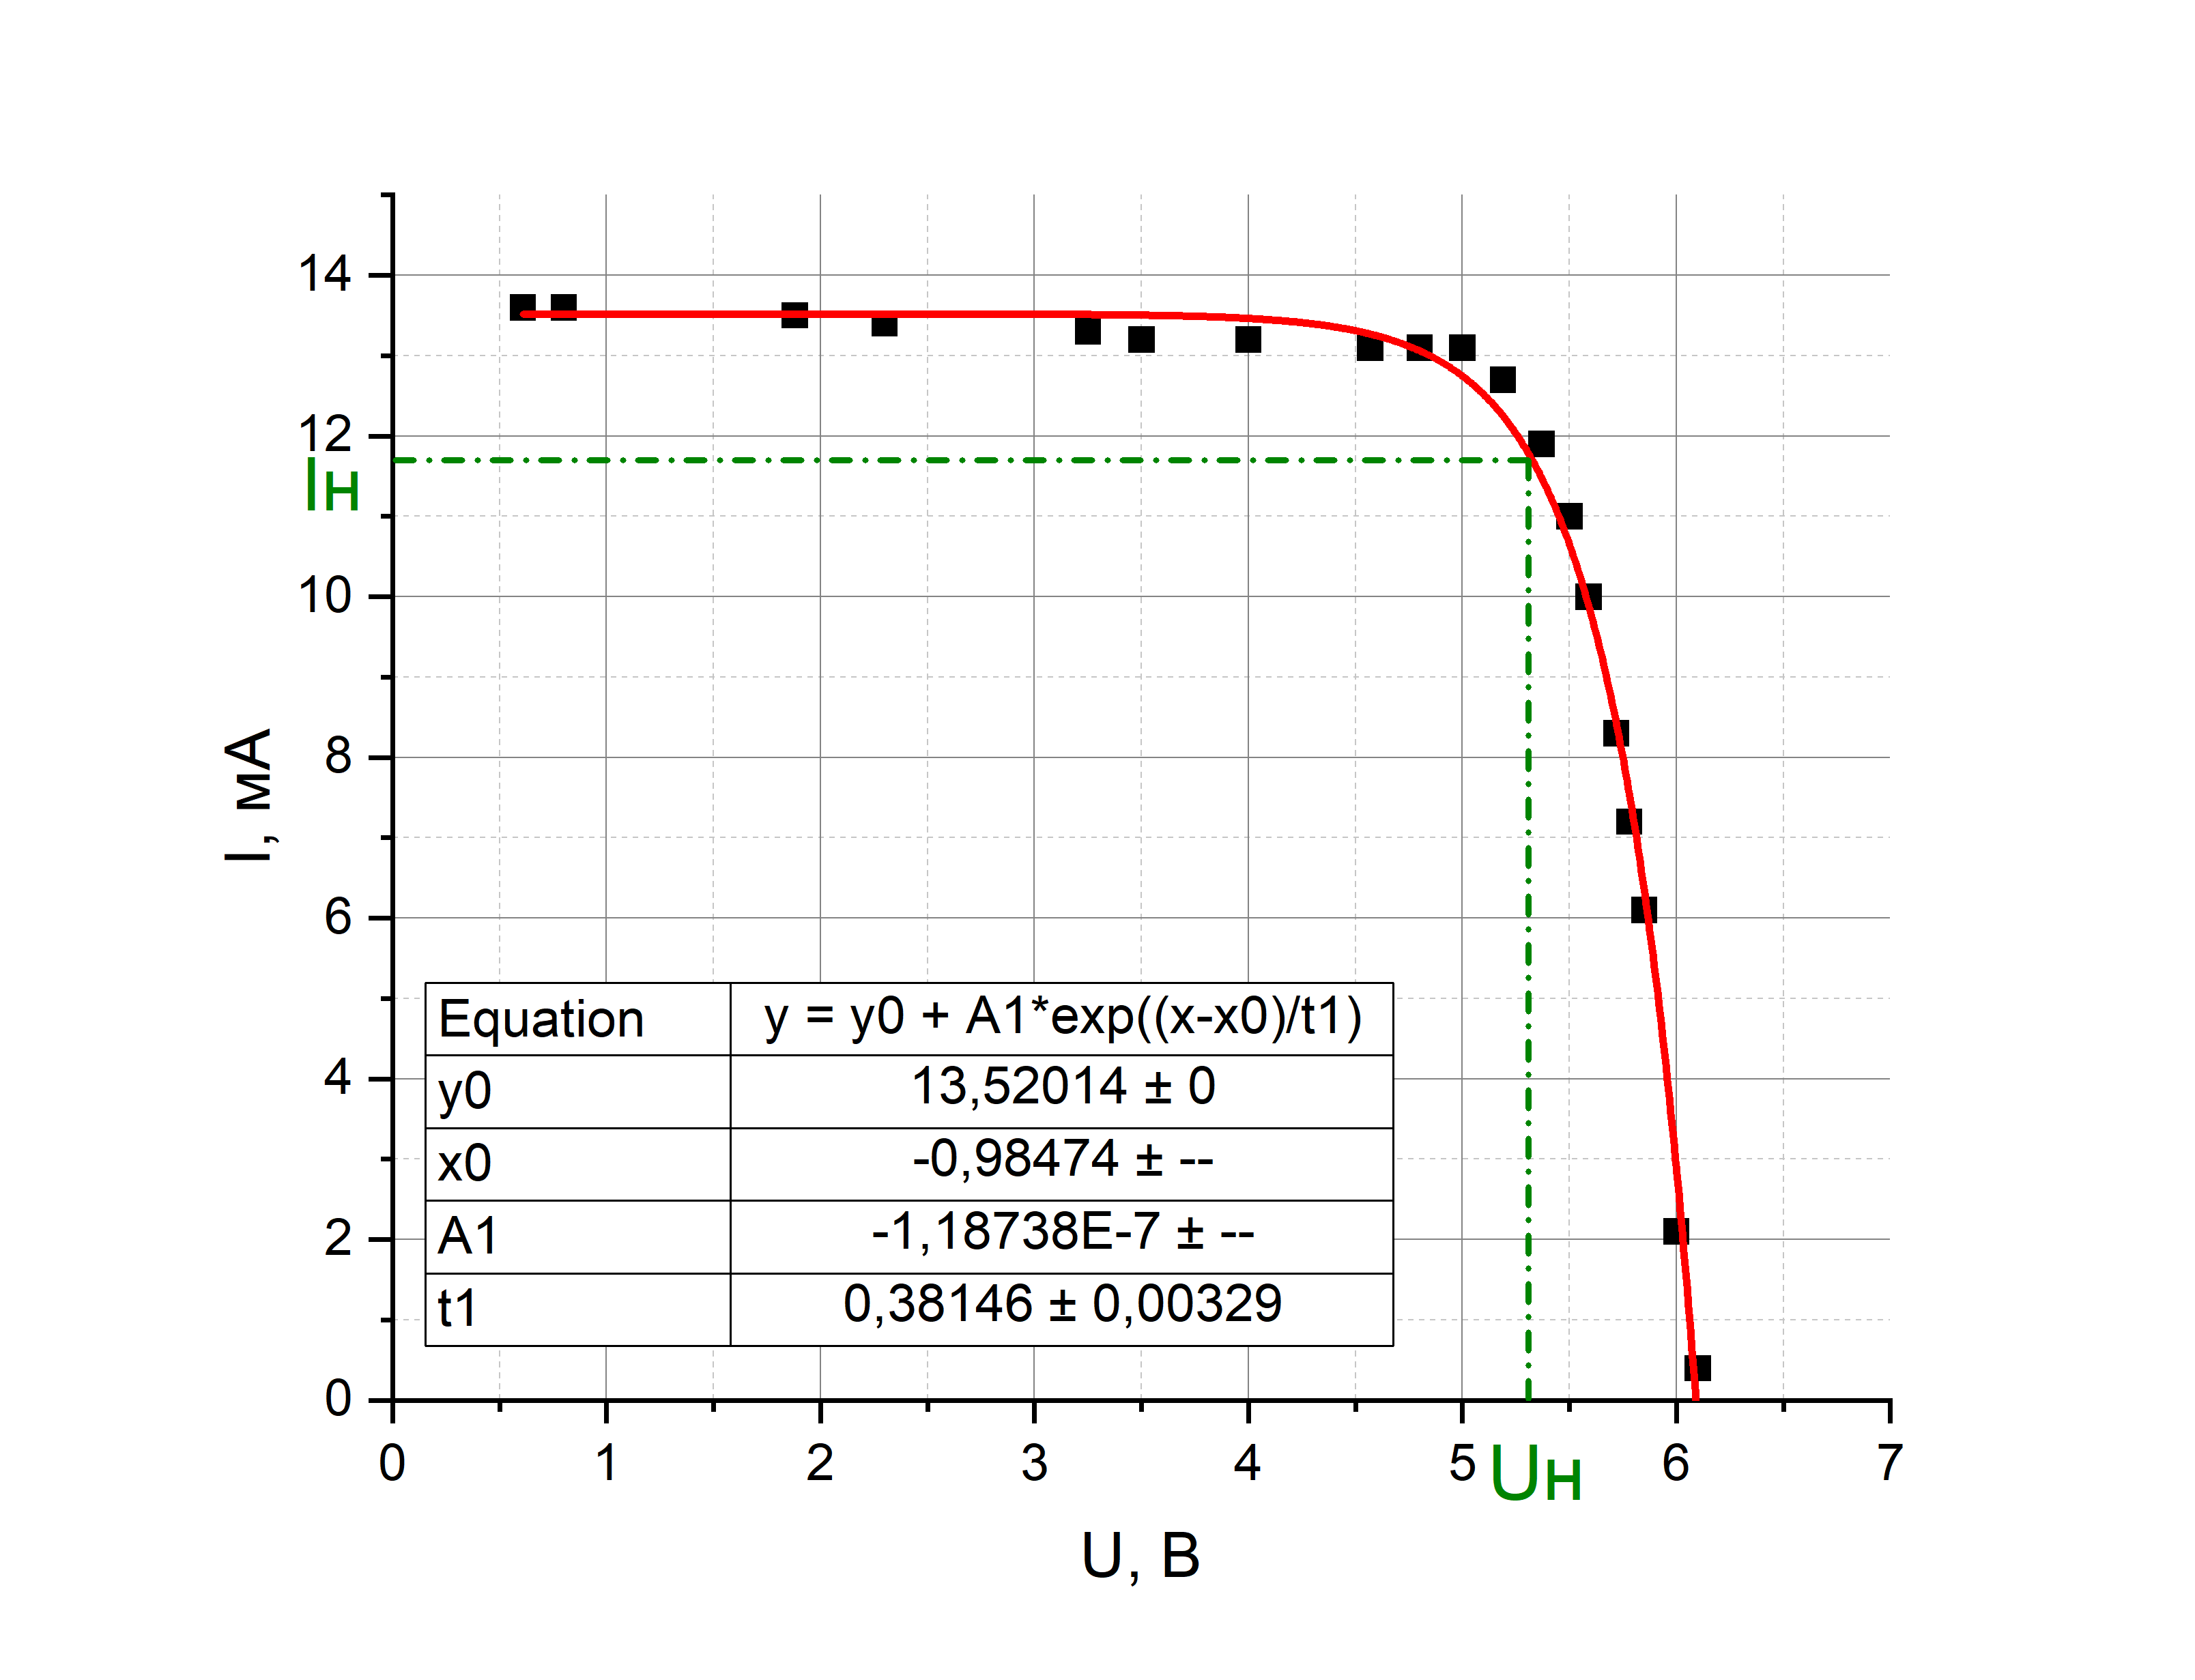
\includegraphics[scale=0.5]{БОЛЬШОЙ Ф-Т прямая световая без фильтра.png}
    \caption{Прямая световая характеристика фотоэлемента без фильтра}
\end{figure}

Аппроксимируем полученную зависимость функцией вида: 
\[
y = y_0 + A_1 e^{\frac{x-x_0}{t_1}}
\]

Получаем ток короткого замыкания, равный коэффициенту $y_0$, $I_{\text{кз}} = 13.5 \pm 0.3 \text{мА}$. 

$U_{xx}$ найдем из условия равенства тока нулю.
\[
0 = y_0 + A_1 e^{\frac{U_{xx}-x_0}{t_1}},
\]

\[
U_{xx} = t_1 \ln\left(\frac{-y_0}{A_1}\right) + x_0 = 5.9 \pm 0.2 \, \text{В}. 
\]

Напряжение нагрузки найдем, построив под кривой прямоугольник наибольшей площади. $U_n = 5.31 \pm 0.2 \, \text{В}$.

Найдём силу тока нагрузки:
\[
I_n = 11.7 \pm 0.2 \, \text{мА}. 
\]

Найдем теперь оптическое сопротивление и мощность преобразователя
\[
R_{\text{опт}} = \frac{U_n}{I_n} \approx 0.5 \, \text{кОм}. 
\]

\[
P = I_n U_n = 69 \pm 2 \, \text{мВт}. 
\]

Из известной мощности падающего излучения $W = 550 \, \text{Вт}/\text{м}^2$ и площади поверхности исследуемого образца $S \approx 60 \, \text{см}^2$ найдём КПД:
\[
\eta = \frac{P}{W S} \approx 0.02.
\]

\subsubsection{Световая характеристика с красным фильтром}


Рассмотрим теперь характеристику, измеренную с красным фильтром.

\begin{figure}[h!]
    \centering
    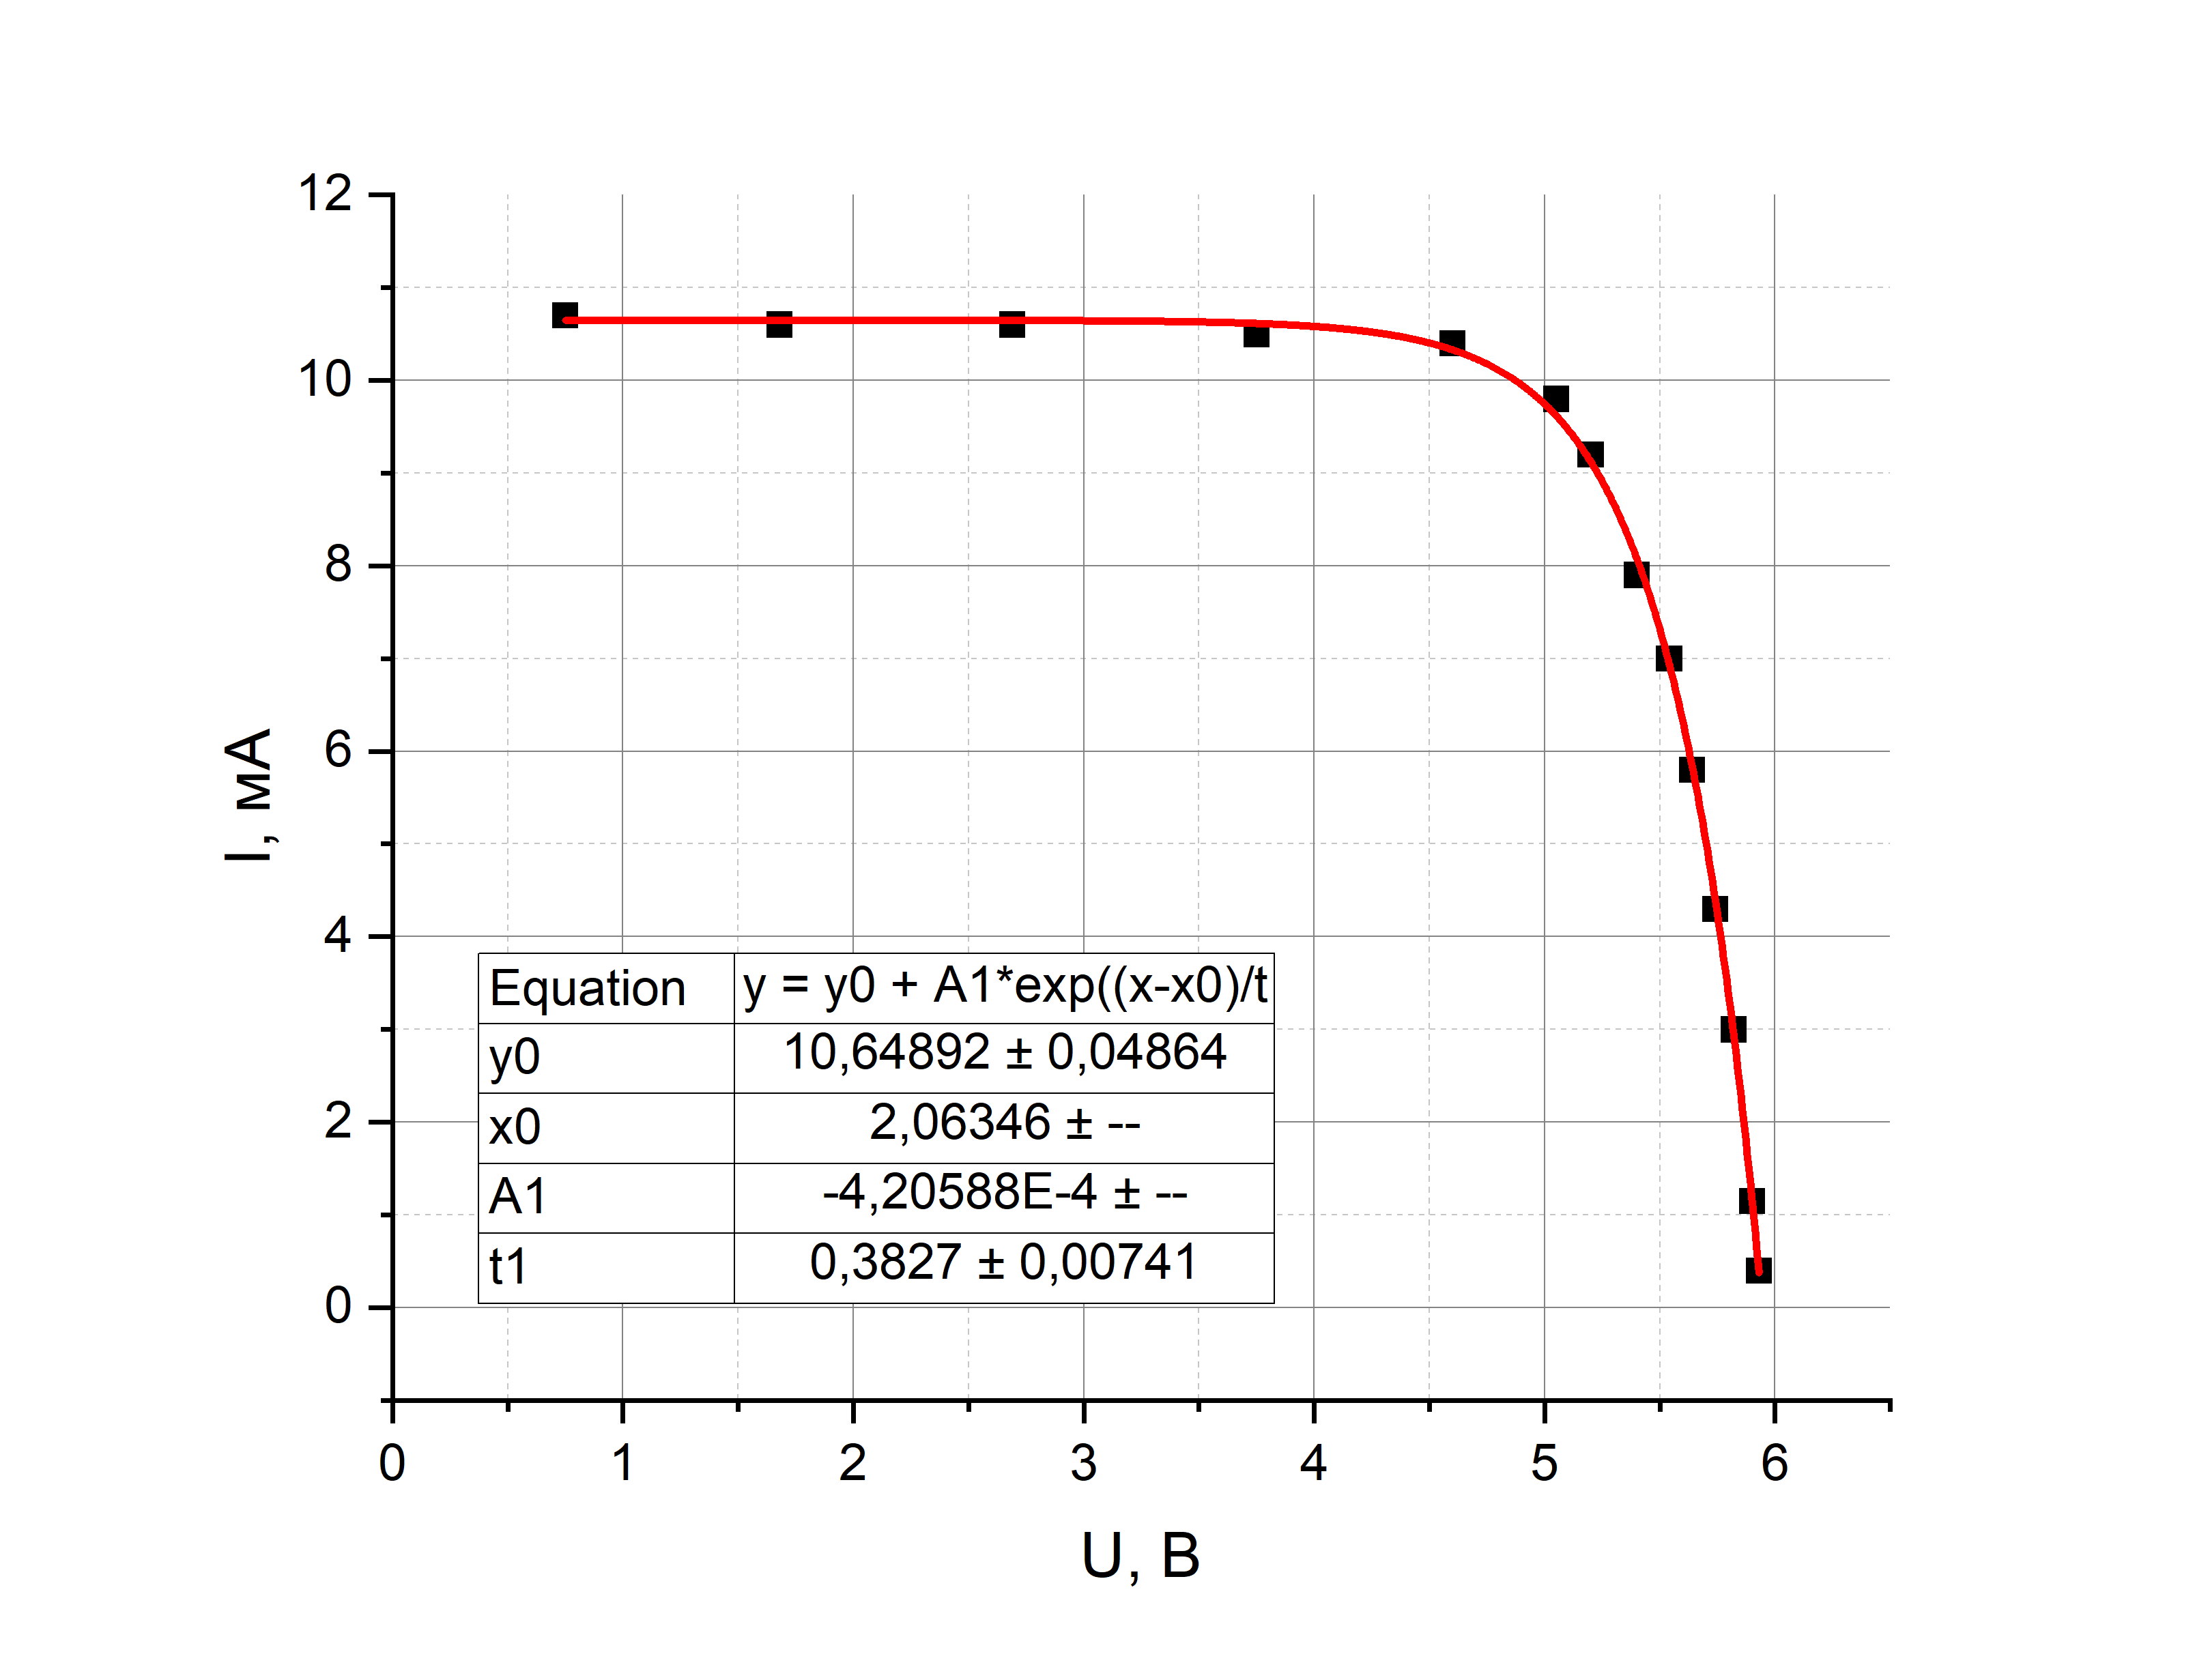
\includegraphics[scale=0.5]{БОЛЬШОЙ Ф-Т прямая световая с фильтром.png}
    \caption{Прямая световая характеристика фотоэлемента с красным фильтром}
\end{figure}

Получим аналогично предыдущему случаю ток короткого замыкания и ЭДС холостого хода:
\[I_{\text{кз}} \approx 10.65 \, \text{мА}, \quad U_{\text{хх}} \approx 4.2 \, \text{В}.
\]

Построим график зависимости $\ln(I_{\text{кз}})$ от $U_{\text{хх}}$. Определим $I_s$ и $A$:
\[
I_s = e^b \approx 0.88 \, \text{мА}. \tag{10}
\]

\[
A = \frac{1}{0.025a} \approx 25.3 \, \frac{1}{\text{мА}}.
\]

\begin{figure}[h!]
    \centering
    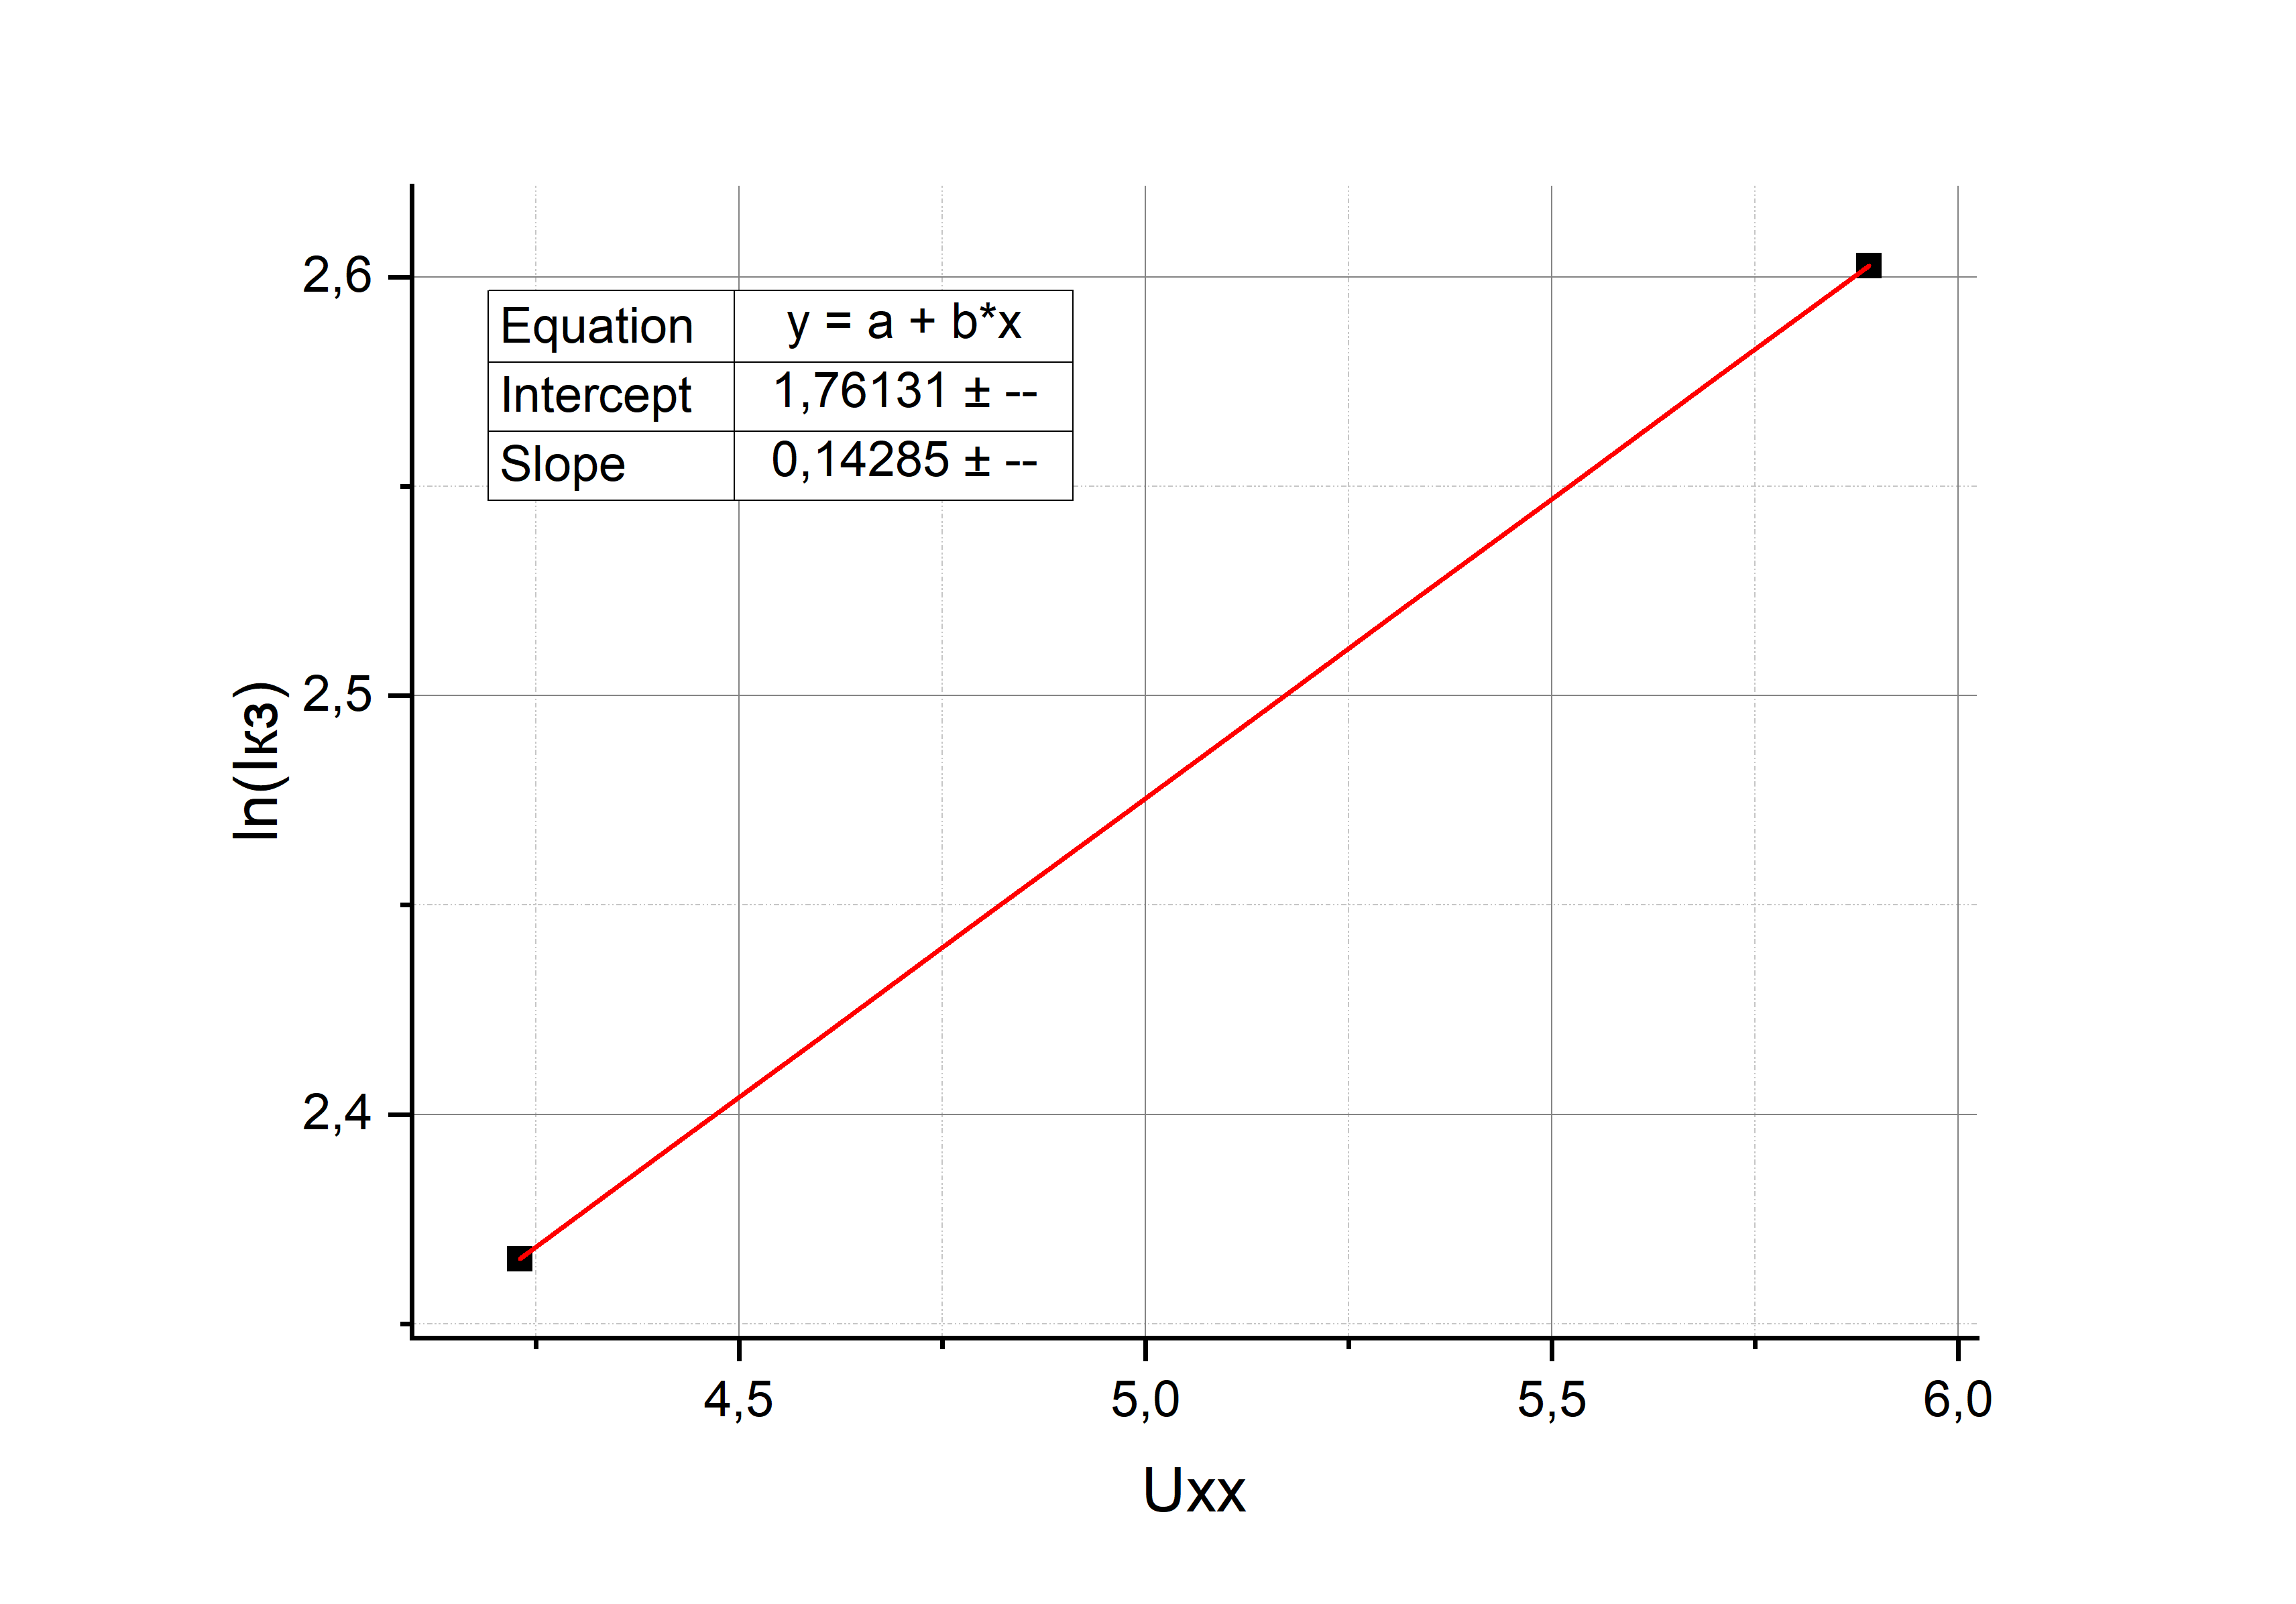
\includegraphics[scale=0.35]{прямая из двух точек.png}
    \caption{Зависимость $ln(I_\text{кз})(U_xx)$}
\end{figure}

\newpage

\section{Вывод}
В ходе работы было изучено явление фотоэффекта в (p-n)-переходе, определены темновая (для фотоэлемента меньшего размера) и световая вольт-амперные характеристики исследуемых фотоэлементов (для фотоэлемента большего размера). Были определены различные параметры: прямое сопротивление, ток и напряжение насыщения, мощность и КПД фотоэлемента.   

Также для фотоэлемента меньшего размера (установка 1) были получены световые характеристики с фильтром и без (рис. 8 и 9).

\begin{figure}[h]
\begin{center}
\begin{minipage}[h]{0.45\linewidth}
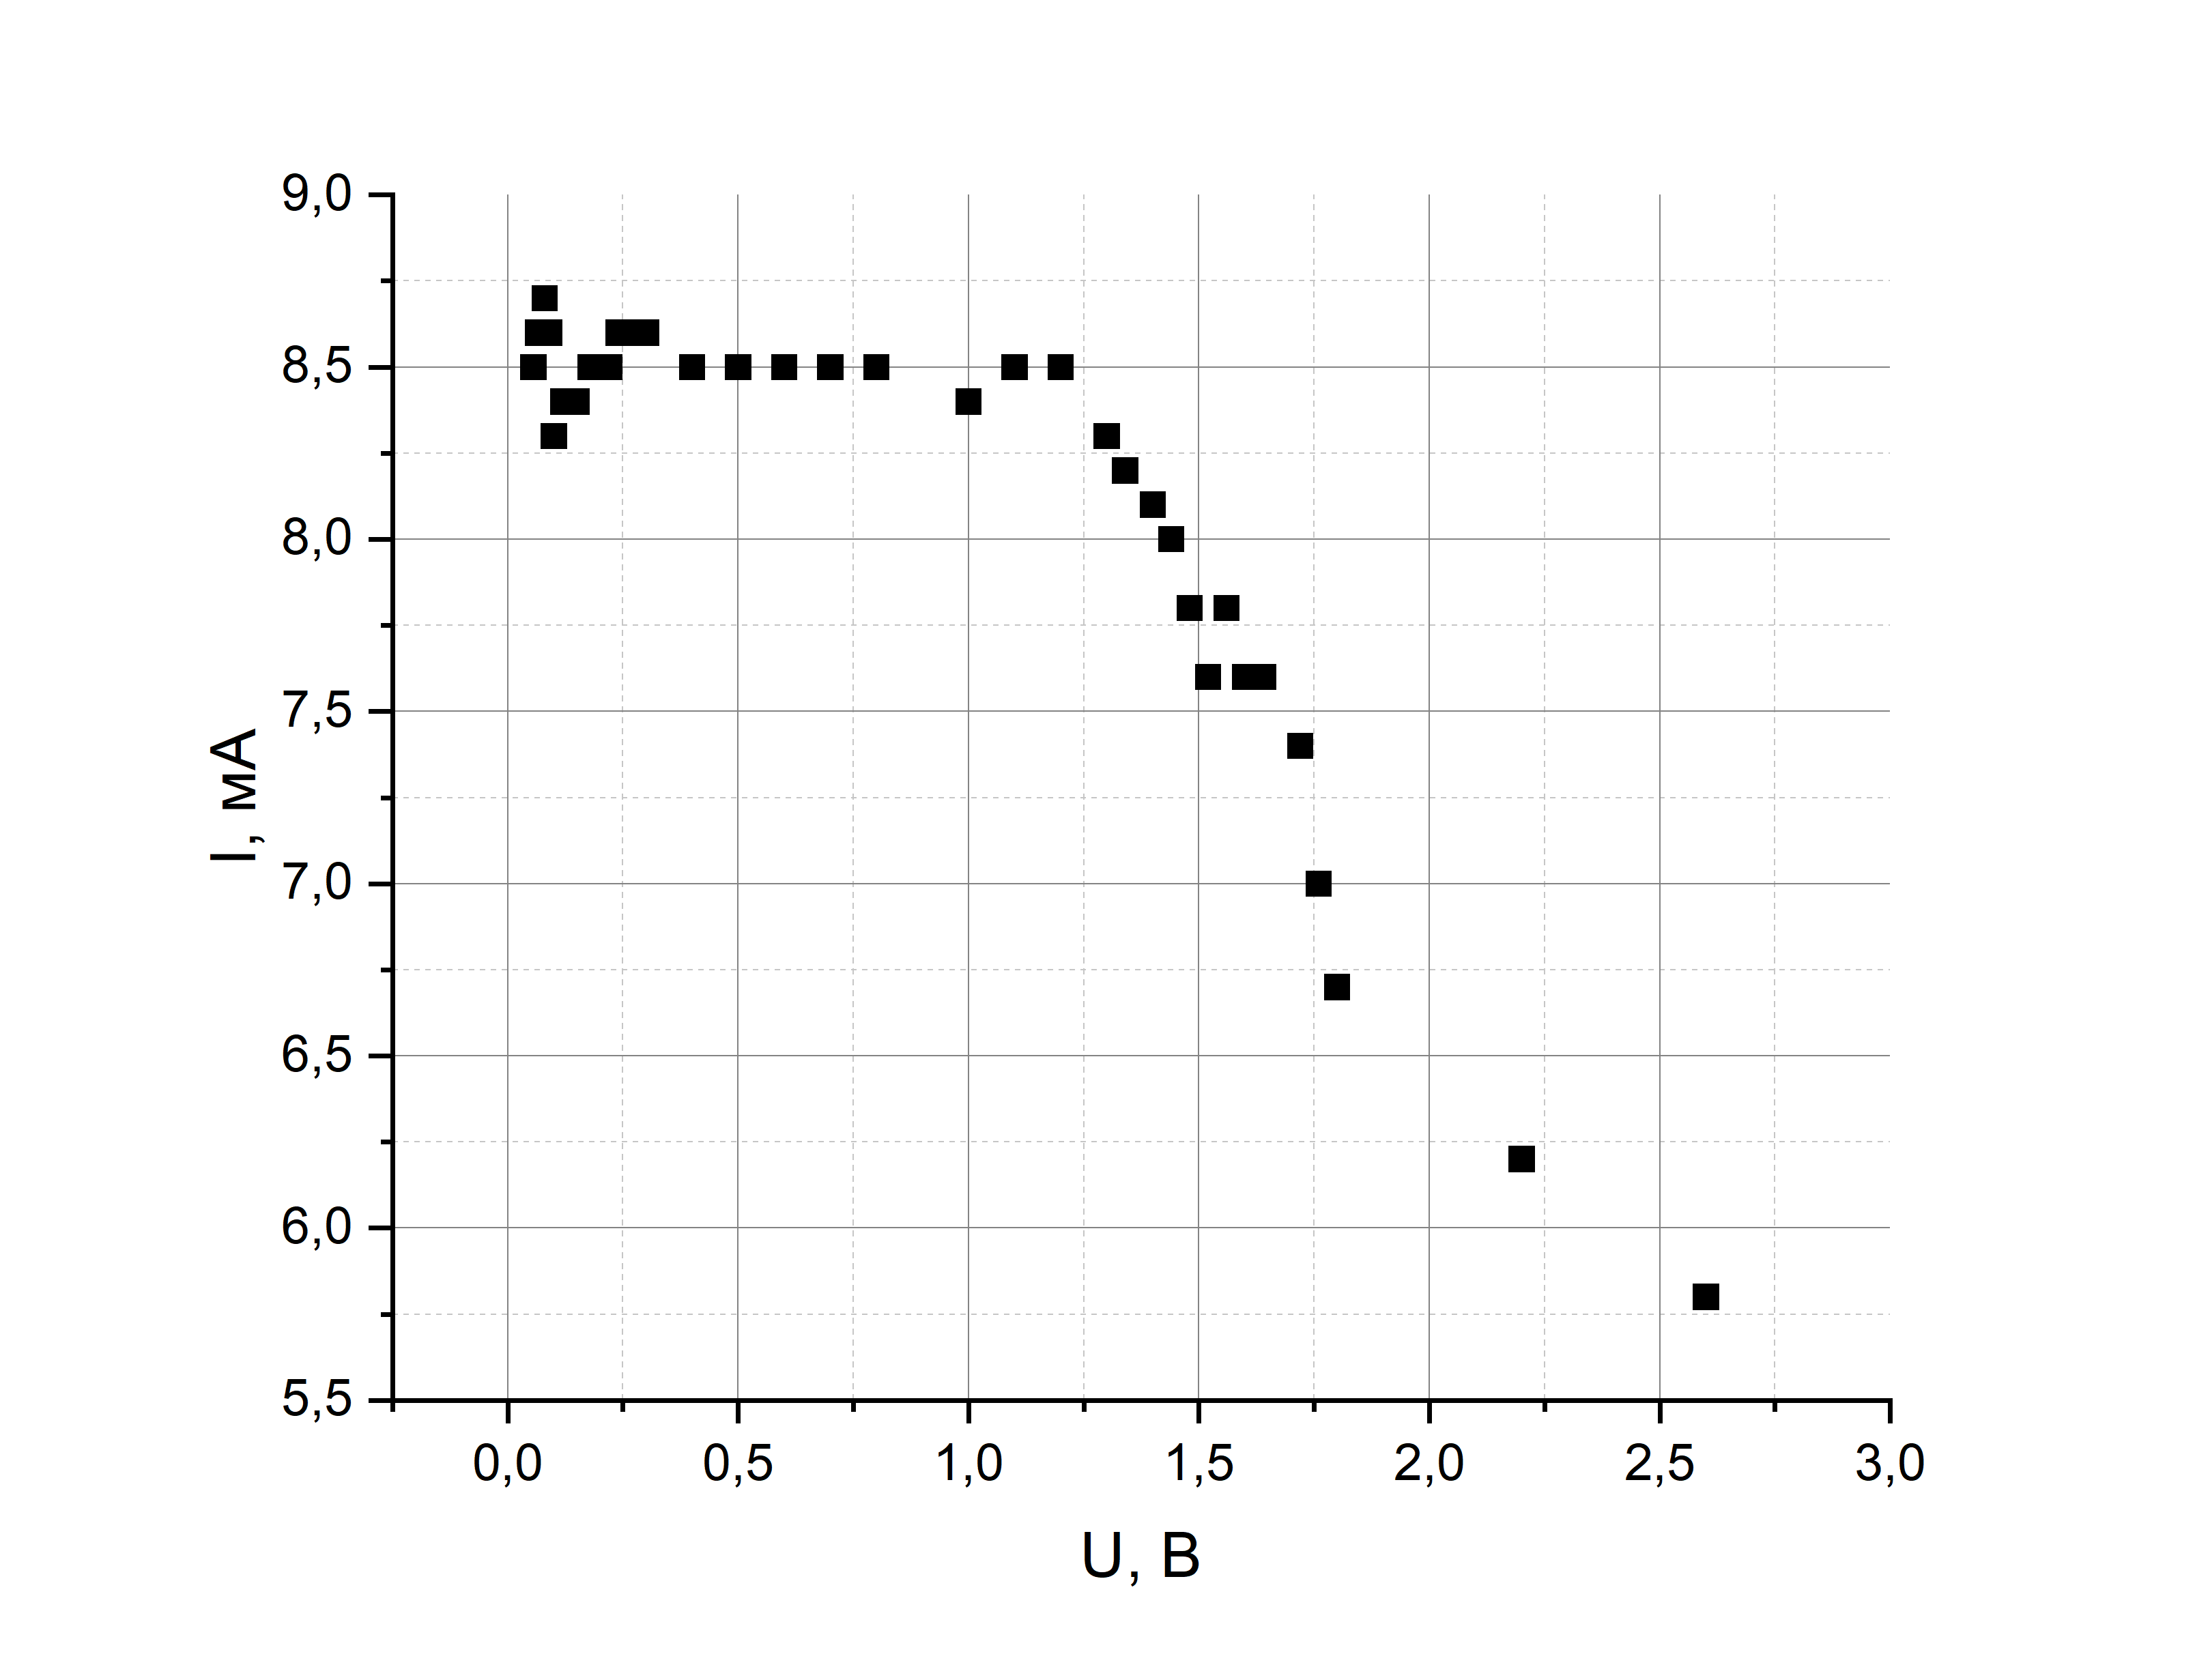
\includegraphics[width=1\linewidth]{прямая световая без фильтра.png}
\caption{Прямая световая характеристика без фильтра для меньшего образца (первая установка)} %% подпись к рисунку
\label{ris:experimoriginal} %% метка рисунка для ссылки на него
\end{minipage}
\hfill 
\begin{minipage}[h]{0.45\linewidth}
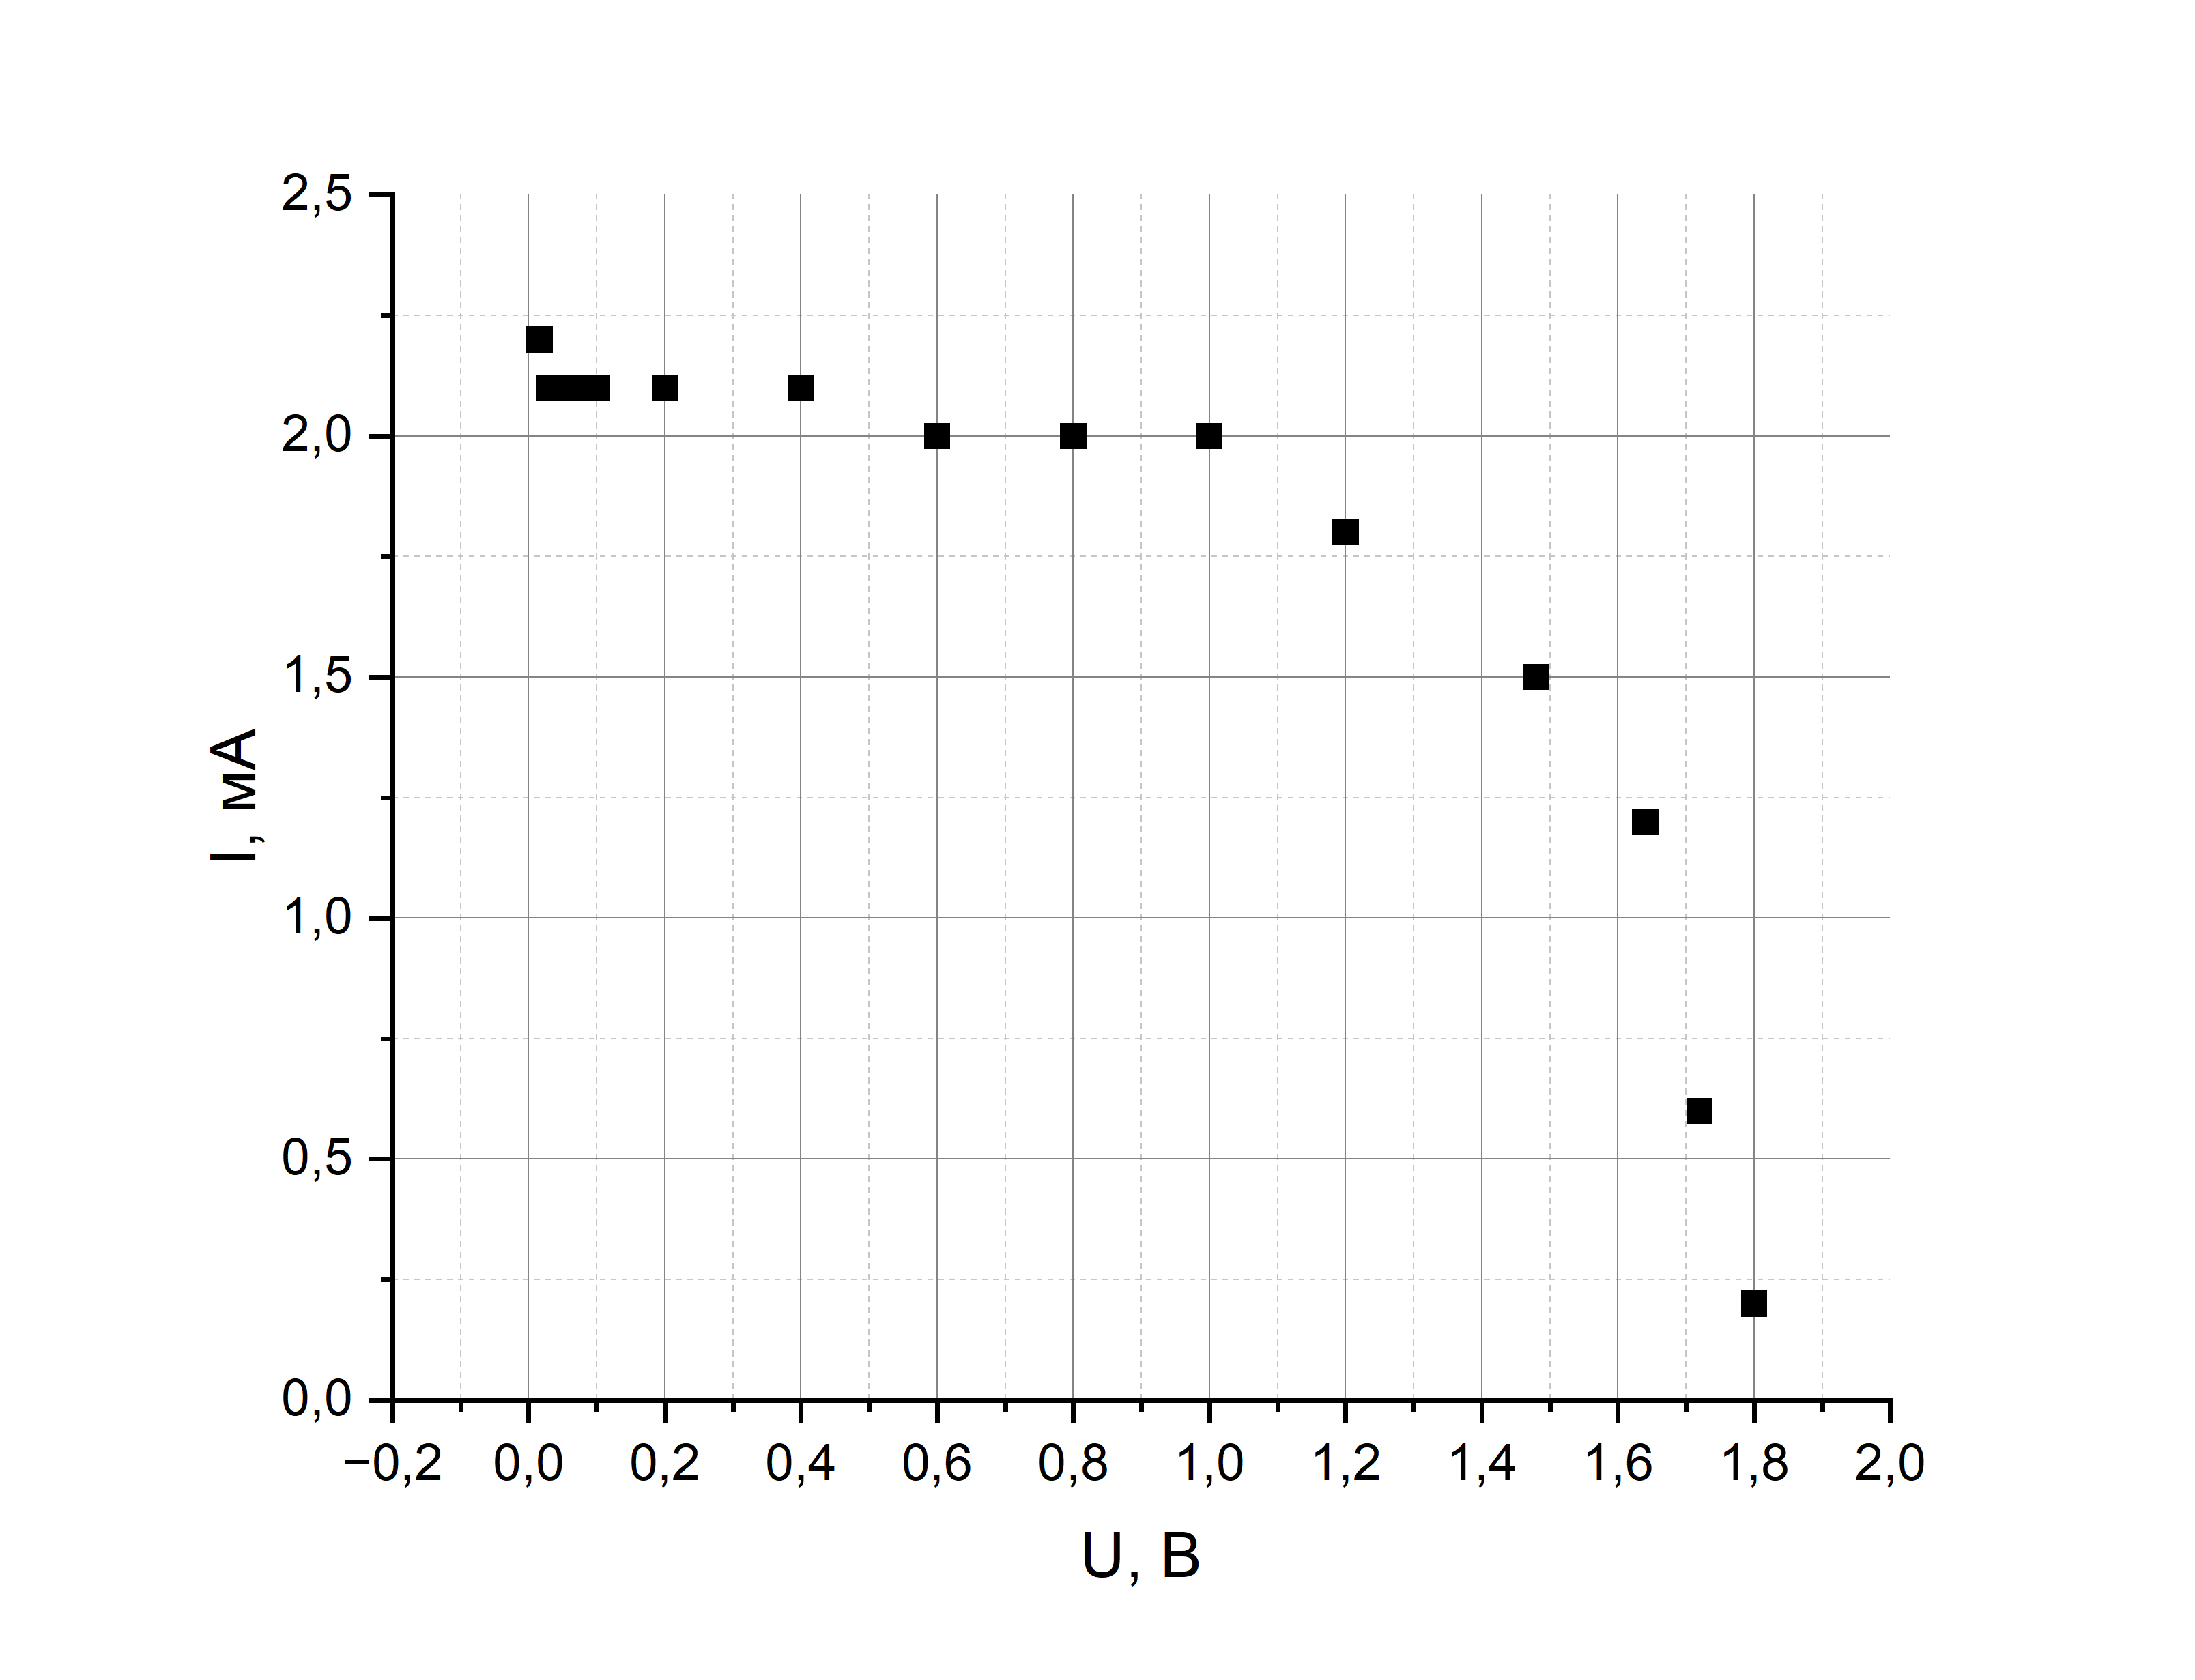
\includegraphics[width=1\linewidth]{прямая световая с фильтром.png}
\caption{Прямая световая характеристика с красным фильтром для меньшего образца (первая установка)}
\label{ris:experimcoded}
\end{minipage}
\end{center}
\end{figure}



\end{document}